% \documentclass[10pt,twoside]{article}
\documentclass{pginz}

\usepackage[utf8]{inputenc}
\usepackage{nicefrac}       % compact symbols for 1/2, etc.
\usepackage{microtype}      % microtypography
\usepackage{ragged2e}
\justifying
\usepackage{float}
\renewcommand{\figurename}{Rysunek}
\usepackage{natbib}
\usepackage{graphicx}
\usepackage{amsmath}
\usepackage{adjustbox}
\usepackage{polski}
\usepackage{gensymb}
\setcitestyle{square}
\usepackage{setspace}
\usepackage{pdfpages}
\usepackage{titlesec}
\usepackage{svg}



\providecommand{\keywordspl}[1]
{
  \small	
  \textbf{\textit{Słowa kluczowe:}} #1
} 
\providecommand{\keywordseng}[1]
{
  \small	
  \textbf{\textit{Keywords:}} #1 
}
\providecommand{\dnauki}[1]
{
  \small	
  \textbf{\textit{Dziedzina nauki i techniki, zgodnie z wymogami OECD:}} #1
}


\begin{document}

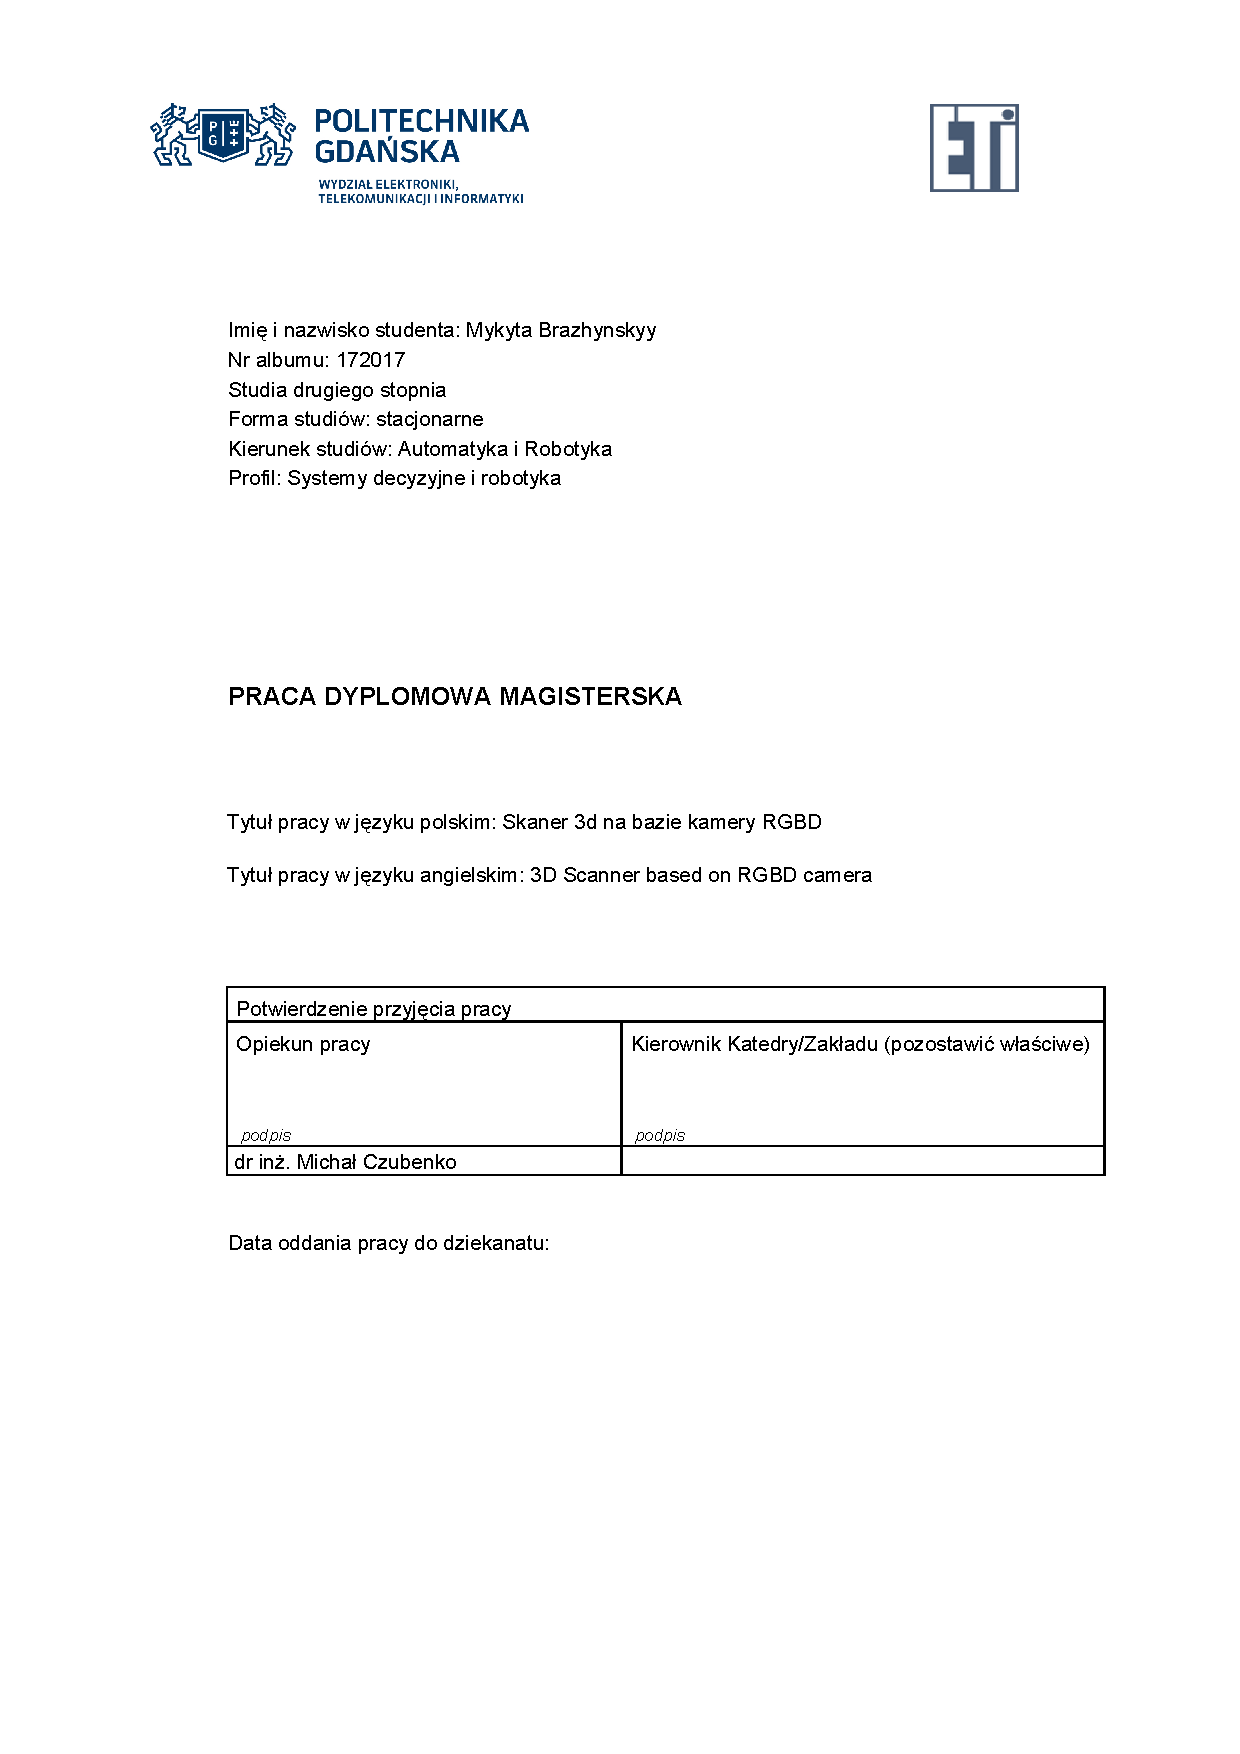
\includepdf[pages=-]{tytolowanowa.pdf}
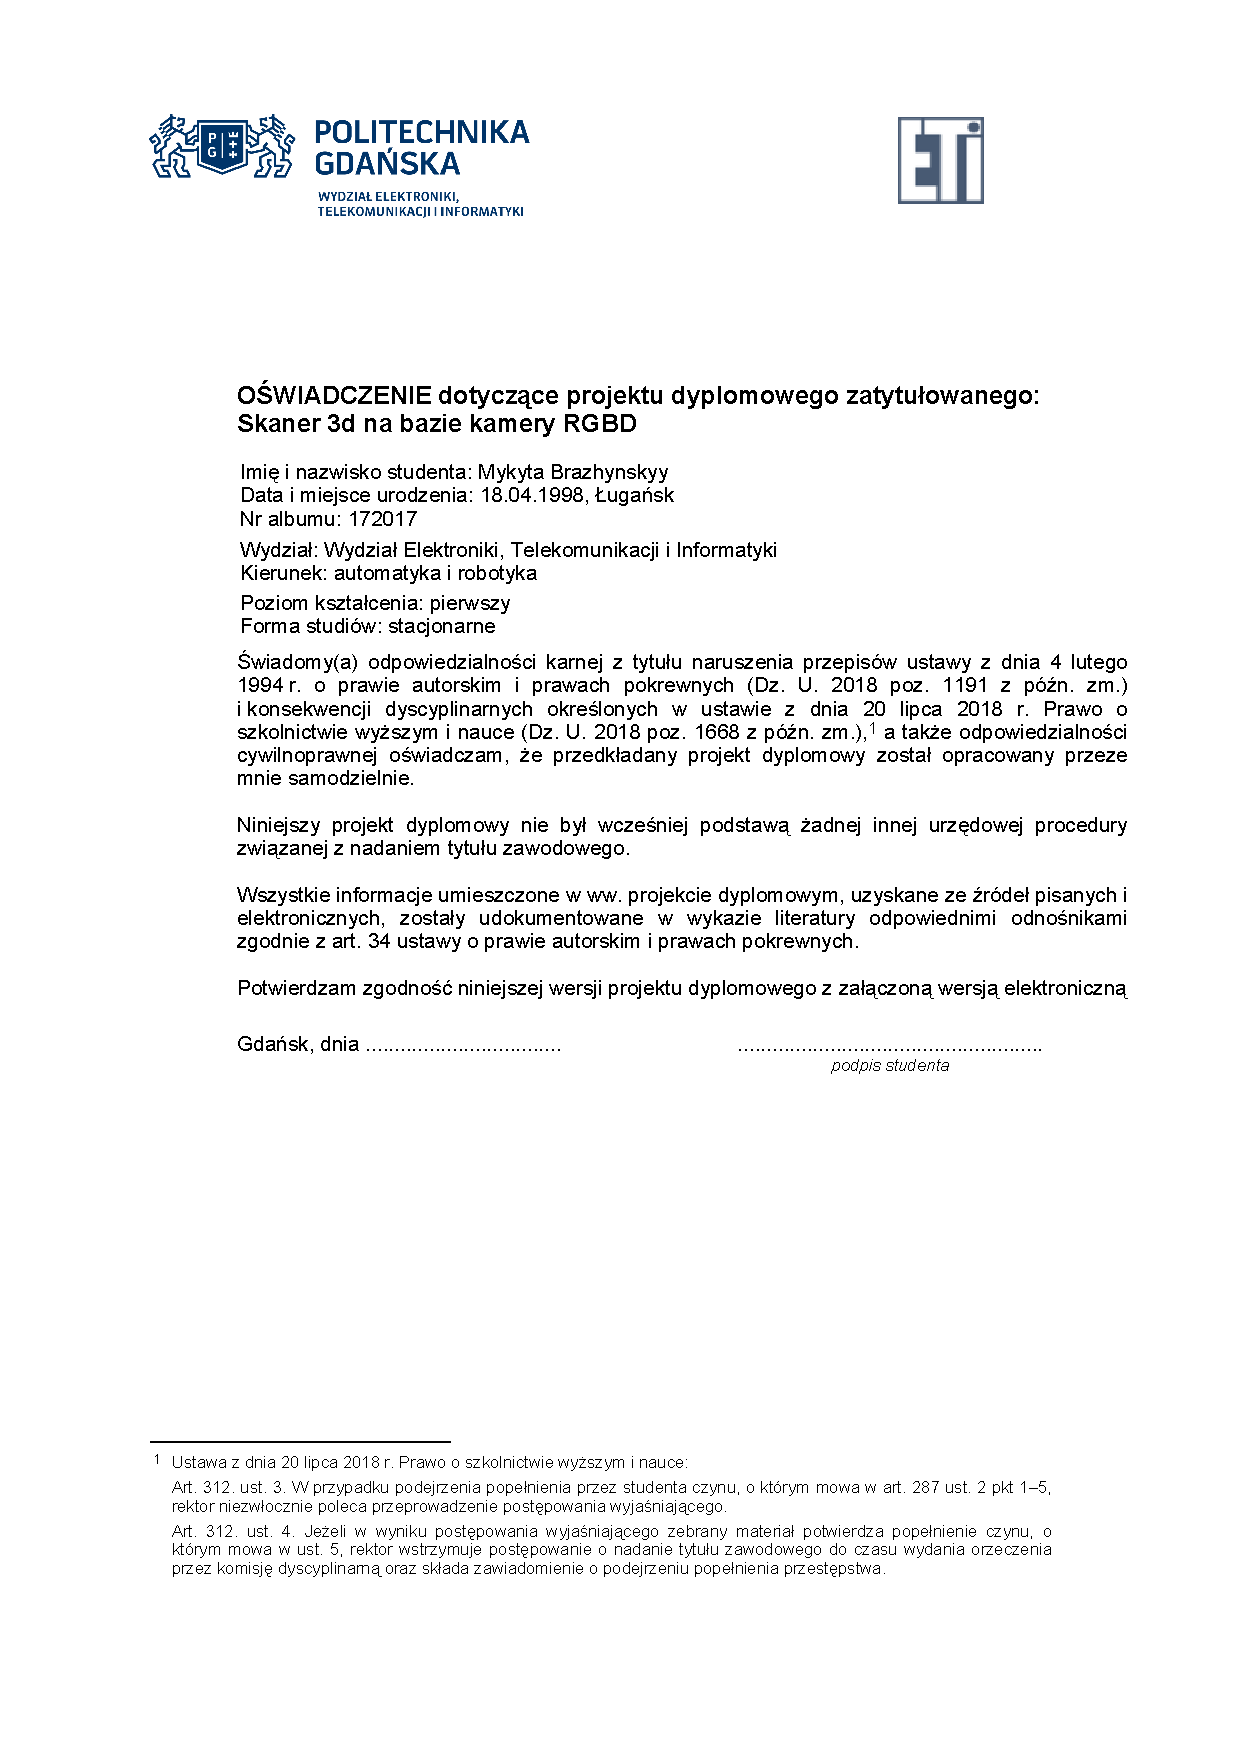
\includepdf[pages=-]{oswiadczenie.pdf}


\setcounter{page}{3}

 
\section*{STRESZCZENIE}
Celem niniejszej pracy dyplomowej było stworzenie skanera 3D oraz systemu wizualizacji utworzonych modeli rzeczywistych obiektów. Do budowy urządzenia wykorzystano kamerę głębi firmy Intel o nazwie RealSense D435i. W pracy został przedstawiony sposób budowy skanera 3D, jego kalibracji oraz algorytmy służące do przetwarzania otrzymanych danych pomiarowych w celu uzyskania wirtualnych modeli. W celu łatwiejszej obsługi programu został utworzony interfejs graficzny zawierający najważniejsze parametry wizualizacji i obróbki danych. Na koniec dane są eksportowane do modeli w formacie obsługiwanym przez program Blender.

\keywordspl{Skaner 3D ,Intel RealSense, Python, Kamera RGBD}

\dnauki{Nauki inżynieryjne i techniczne, Systemy automatyzacji i kontroli }

\section*{ABSTRACT}
The aim of this thesis was to create a 3D scanner and a system for visualization of created models based on real objects. In the work is presented how to build a 3D scanner, its calibration and algorithms used to process the obtained measurement data to obtain virtual models. In order to make the program easier to use, a graphic interface was created containing the most important parameters of visualization and data processing. Finally, the data are exported to the models in a format supported by the Blender program.

\keywordseng{3D Scanner, Intel RealSense, Python, RGBD Camera}
\newpage
\tableofcontents


\newpage

\chapter*{WYKAZ WAŻNIEJSZYCH OZNACZEŃ I SKRÓTÓW}
\subsection*{RGB}
Paleta barw tworząca kolor piksela. Oznaczenie pochodzi od kolorów Red, Green, Blue czyli czerwony, zielony, niebieski.
\subsection*{Kamera RGBD}
Kamera głębi, oprócz wykonywania zdjęć RGB potrafi ona również dokonać pomiaru odległości od obiektów i nanieść te informację na powierzchnię poszczególnych pikseli obrazu.
\subsection*{LIDAR}
Ang.(Light Detection And Ranging) urządzenie służące do dokładnego pomiaru odległości. Działaniem przypomina funkcjonowanie radaru, lecz korzysta z odliczania czasu przelotu światła lasera, a nie mikrofal.
\subsection*{Blender}
Oprogramowanie służące do modelowania trójwymiarowego.Posiada szereg funkcji do animacji obiektów, generacji tekstur oraz importowania i eksportowania gotowych modeli.
\subsection*{Maya}
Program komputerowy, umożliwiający generację zaawansowanych modeli 3D przeznaczony do zastosowań przemysłowych. W tym programie zostały stworzone filmy takie jak Spiderman, Avatar oraz Up.
\subsection*{LIDAR}
Skaner impulsowy LIDAR jest urządzeniem mierzącym odległość za pomocą wiązki światła. Jego zasada działania jest zbliżona do funkcjonowania radaru.
\chapter{WSTĘP I CEL PRACY}
\section{Wprowadzenie}
W bieżącym rozdziale przedstawione zostaną wyniki implementacji dwóch metod rekonstrukcji powierzchni z chmury punktów. Omówione zostaną charakterystyki poszczególnych algorytmów oraz rezultaty dzięki nim uzyskane. Ukazana zostanie implementacja wybranego z nich.
W celu uzyskania trójwymiarowych modeli na podstawie skanów rzeczywistych obiektów, przetestowano dwie metody generacji meshu. Pierwszą z nich jest ball pivoting algorithm. Kolejnym algorytmem będzie trójwymiarowa triangulacja Delaunay'a.


\section{Cele i założenia}
Celem niniejszej pracy jest zaprojektowanie skanera 3D korzystającego z metody triangulacji laserowej  oraz wyeksportowanie modeli do programu Blender przy zastosowaniu kamery RGBD. Projekt składa się z dwóch części, budowy skanera trójwymiarowego oraz stworzenie programu do obróbki otrzymanych danych. Odległość z jakiej będzie wykonywany skan wynosi do 1 m. Powyżej tej wartości gęstość punktów będzie zbyt niska do wiernego odtworzenia modelu. Czas trwania obliczeń w programie wynosi poniżej 15 minut. Utworzony model powinien jak najwierniej oddawać wygląd rzeczywistego obiektu, luki w teksturze powinny nieznacznie wpływać na ostateczny wygląd.

\section{Zawartość pracy}
Pierwszy rozdział opisuje cele oraz założenia pracy.Dokonano gruntownej analizy problemu, który zostanie rozwiązany w dalszym ciągu pracy.

W drugim rozdziale wykonano przegląd istniejących metod mających na celu generację trójwymiarowych obiektów na podstawie danych z kamery głębi. Dokonano porównania pomiędzy dostępnymi na rynku skanerami 3D bazującymi na różnych technologiach pomiarowych. Wymieniono ich parametry techniczne. Zobrazowano w jakich warunkach dana metoda pomiarowa powinna zostać wykorzystana. Ukazane zostały również technologie jakimi posługiwano się w przeszłości do generacji trójwymiarowych modeli. Na koniec przedstawione zostały zastosowania współczesnych skanerów 3D.

W kolejnym rozdziale przedstawiony jest model oraz konstrukcja skanera 3D. Wyjaśniono metody służące do przetworzenia danych uzyskanych z kamery głębi w chmurę punktów. Przedstawiono koncepcje istniejących rozwiązań służących do rekonstrukcji powierzchni oraz kształtu obiektów z chmury punktów.

Czwarty rozdział przedstawia podsumowanie zarówno wykonanej pracy, jak i otrzymanych efektów. Ukazane zostaną również metody analizy oraz obróbki danych, które mają posłużyć do cyfrowej implementacji rzeczywistych obiektów zarejestrowanych przez kamerę RGBD. Przedstawiono opisy zastosowanych algorytmów oraz kolejność ich wykonywania na podstawie autorskiego programu w języku Python. Poddano analizie pod względem dokładności rezultaty pomiarów w porównaniu do rzeczywistych wartości mierzonych.

Ostatni rozdział porusza kwestię potencjalnych możliwości udoskonalenia urządzenia.

\section{Wprowadzenie}
W bieżącym rozdziale przedstawione zostaną wyniki implementacji dwóch metod rekonstrukcji powierzchni z chmury punktów. Omówione zostaną charakterystyki poszczególnych algorytmów oraz rezultaty dzięki nim uzyskane. Ukazana zostanie implementacja wybranego z nich.
W celu uzyskania trójwymiarowych modeli na podstawie skanów rzeczywistych obiektów, przetestowano dwie metody generacji meshu. Pierwszą z nich jest ball pivoting algorithm. Kolejnym algorytmem będzie trójwymiarowa triangulacja Delaunay'a.


\begingroup
\newpage

\let\clearpage\relax
\chapter{Model skanera oraz koncepcja działania}
\section{Wprowadzenie}
W bieżącym rozdziale przedstawione zostaną wyniki implementacji dwóch metod rekonstrukcji powierzchni z chmury punktów. Omówione zostaną charakterystyki poszczególnych algorytmów oraz rezultaty dzięki nim uzyskane. Ukazana zostanie implementacja wybranego z nich.
W celu uzyskania trójwymiarowych modeli na podstawie skanów rzeczywistych obiektów, przetestowano dwie metody generacji meshu. Pierwszą z nich jest ball pivoting algorithm. Kolejnym algorytmem będzie trójwymiarowa triangulacja Delaunay'a.


\section{Model i konstrukcja skanera 3D}
W celu wykonania dokładnych modeli trójwymiarowych został utworzony skaner 3D na podstawie autorskiego projektu. W skład zestawu wchodzi kamera Intel RealSense D435i oraz platforma ruchoma. Wybór sensora od firmy Intel nie był przypadkowy. Posiada on szereg wbudowanych funkcji, takich jak łatwa możliwość kalibracji oraz nastaw odpowiednich parametrów wykrywania głębi. Podczas budowy skanera dokonano porównania możliwości dwóch kamer trójwymiarowych: Intel RealSense D435i oraz Orbbec Astra Mini MX6000. Porównanie charakterystyk tych produktów znajduje się w tabeli ~\ref{tab:intelvsorbbec}.

\begin{table}[H]
\begin{center}

\caption{\label{tab:intelvsorbbec}Porównanie charakterystyk kamer Intel RealSense D435i oraz Orbbec Astra Mini MX6000 \cite{OrbbecAstraMiniSheet} \cite{IntelRealSenseSheet}.}
\centerline{
\begin{tabular}{ |c| c|c| }
 \hline
 {\small Kamera} & {\small Astra Mini} & {\small RealSense D435i}\\ 
 \hline
 {\small Dokładność} & {\small $\pm$ 1-3mm na 1 m} & {\small < \text{2\%}  na 2 m}\\ 
  \hline
   {\small FOV} & {\small 60 \degree H x 49.5 \degree V} & {\small 87 \degree H x 58 \degree V}\\ 
  \hline
 {\small Rozdzielczość RGB } & {\small 640 px x 480 px } & {\small 1920 px x 1080 px}   \\  
  \hline
   {\small Rozdzielczość głębi } & {\small 640 px x 480 px } & {\small 1280 px x 720 px }   \\  
  \hline
     {\small FPS } & {\small 30} & {\small 90}   \\  
  \hline
   {\small  Długość fali lasera } & {\small 830 nm} & {\small 850 nm}  \\  
  \hline


\end{tabular}
}

\end{center}
\end{table}
Z powyższych charakterystyk wynika, że kamera firmy Intel jest dokładniejsza oraz lepiej spełni zadanie wiernego odwzorowania modelu 3D. Ponadto oprogramowanie dostarczane przez firmę Intel o nazwie RealSense Viewer pozwala na łatwą obsługę tego urządzenia. Jest tam możliwość podglądu obrazu z kamery zarówno w 2D jak i w 3D. Można ustawić poszególne parametry niezbedne do poprawnej rejestracji obrazu takie jak moc lasera, wartość graniczną wykrywanej głębi oraz ekspozycję. Wszystkie te aspekty znacząco usprawniają proces kalibracji,produktywność oraz wpływają na poprawę dokładności generowanych obrazów.
Konstrukcja zbudowanego skanera została zaprezentowana na rysunku ~\ref{fig:konstrukcjaModelu}. 
\begin{figure}[H]
  \centering
    \includesvg[scale=0.75]{modelSkanera.svg}

  \caption{Schemat budowy autorskiego skanera 3D.}   
  \label{fig:konstrukcjaModelu}
\end{figure}
Na powyższym rysunku dostrzec można dostrzec dwa kluczowe elementy wchodzące w skład skanera. Platforma ruchoma napędzana silnikiem elektrycznym zapewnia stałą prędkość kątową obrotu tacki. Dzięki temu wyznaczanie położenia obiektu w przestrzeni jest dokładne. Wykonane zostały testy platformy napędzanej silnikiem elektrycznym oraz tej poruszanej ręcznie. Z wytworzonych w ten sposób modeli wynika jasno, iż stała prędkość kątowa obiektu jest kluczowa do poprawnego przekształcenia modelu. Kolejnym elementem wykorzystanym przy budowie skanera jest kamera RGBD. Wykonuje ona zdjęcia RGB oraz głębi z określoną częstotliwością oraz zapisuje je do pliku, w celu późniejszej ich obróbki. Dokonane zostało porównanie wpływu FPS na wygląd ostatecznego modelu. Bezpośrednio wpływa to na rozdzielczość kątową wykonanych zdjęć, a co za tym idzie, zmniejszenie gęstości chmury punktów.\\
Skaner funkcjonuje w następujący sposób:
\begin{enumerate}
    \item Mierzona jest dokładna odległość obiektywu kamery od środka tacki.
    \item Obiekt umieszczany jest na obrotowej tacce.
    \item Dokonuje się kalibracji tak ustawionego elementu, tak by stopień wypełnienia punktów był jak najdokładniejszy.
    \item Tacka zostaje uruchomiona z prędkością 0.1 $\frac{rad}{s}$.
    \item Uruchomiony zostaje zapis obrazu głębi oraz RGB z kamery.
    \item Gdy tacka wykona pełen obrót, nagrywanie oraz tacka zostają zatrzymane.
\end{enumerate}

Wysokość obiektu jest mierzona na podstawie danych z kamery RGBD. Znając odległość kamery od obiektu, można wyznaczyć jego wysokość korzystając ze wzoru.

\begin{equation}
    \begin{aligned}
        H=\frac{163.6}{3.7 \cdot D} -10.6
    \end{aligned}
\end{equation}

Powyższy wzór został wyznaczony metodą empiryczną. W tym celu zmierzono wysokość obiektu na obrazie kamery oraz odległość od tego obiektu od obiektywu. Badanie powtórzono dwanaście razy w celu uzyskania dokładnej liniowej aproksymacji. Następnie wyznaczona została linia najlepszego dopasowania, wykorzystując również informację o tym, że powinna to być zależność odwrotnie proporcjonalna. Wykres przedstawiający zmierzone punkty oraz linię będącą wynikiem metody najmniejszych kwadratów ukazany na rysunku ~\ref{fig:wysokoscOdleglosc}.
\begin{figure}[H]
  \centering
    \includesvg[scale=0.75]{wysokosc_odleglosc}

  \caption{Zależność wysokości w pikselach od odległości kamery od obiektu.}   
  \label{fig:wysokoscOdleglosc}
\end{figure}

\section{Przejście do chmury punktów}
Przypomnieć zasade działania skanera i jak to wykorzystujemy. Tutaj pokazujemy na jakiej zasadzie następuje przejście z płaszczyzny 2D do 3D.Dać obrazek zastosowanej metody oraz równania.

Metoda przejścia w chmurę punktów na podstawie danych z kamery RGBD składa się z kilku kroków. Poniżej zostały opisane procedury, które należy wykonać w celu otrzymania wyżej wymienionego rezultatu.
\subsection{Wstępna obróbka danych.}
Pierwszym krokiem użytej metody jest wstępna obróbka danych. Odczytywane są dane zapisane w pliku .bag z kamery RGBD. Następnie, wybierana jest kolumna obrazu która posłuży do ekstrakcji danych z kamery głębi. Filtracja w ten sposób danych ma na celu zwiększenie wydajności kodu. Dzieje się tak, ponieważ do późniejszych algorytmów będzie wykorzystywana tylko jedna kolumna z klatki obrazu,a nie cały obraz.

\subsection{Przekształcenie danych z kamery RGBD do współrzędnych 3D.}
Następnym etapem schematu jest przejście z dwuwymiarowego układu współrzędnych kamery do trójwymiarowego układu obiektu. W tym celu zostanie użyte poniższe przekształcenie, wynikiem którego będzie macierz czterowymiarowych punktów. W skład punktu wchodzą trzy współrzędne odpowiadające pozycji w przestrzeni oraz wartość RGB danego punktu symbolizująca jego kolor.

\begin{equation}
    \begin{aligned}
            & D_{\beta}=\begin{bmatrix}d_{0} & \dots & d_{max} \end{bmatrix}  \\
            & RGB_{\beta}=\begin{bmatrix}rgb_{0} & \dots & rgb_{max} \end{bmatrix}  \\
            & X_{\beta}=cos(\beta)(R-D_{\beta})  \\
            & Y_{\beta}=sin(\beta)(R-D_{\beta})  \\
          & Z=\begin{bmatrix} 0 & \dots & H_{max} \end{bmatrix}  \\
          & w_{\beta}^n=\begin{bmatrix} X_{\beta}[n] & Y_{\beta}[n] & Z[n] & RGB_{\beta}[n]\end{bmatrix}  \\
    \end{aligned}
    \label{equ:chmuraPunktow}
\end{equation}

$\beta$ jest kątem obrotu tacki. R jest odległością obiektywu kamery od środka osi obrotu tacki. $D_{\beta}$ to macierz zmierzonych odległości punktów na płaszczyźnie obiektu od kamery dla danego kąta obrotu $\beta$. $X_{\beta}$,$Y_{\beta}$ są macierzami współrzędnych punktów na osi X,Y dla nago kąta $\beta$. $H_{max}$ to wysokość obiektu. Z to macierz współrzędnych punktów na osi Z. Wypełniona jest ona punktami z zakresu od 0 do $H_{max}$. $w_{\beta}^n$ to współrzędne n-tego punktu w płaszczyźnie XYZ dla danego kąta obrotu $\beta$.

\subsection{Normalizacja otrzymanych punktów.}
Kamera RGBD jest zaawansowanym technicznie urządzeniem. Pomimo kalibracji kamery, w przechwyconych obrazach mogą występować niedoskonałości. Przejawiają się one w złych pozycjach punktów względem pozostałych wartości. Jest to spowodowane błędnymi odczytami głębi poprzez sensor kamery i jest nieuniknione. Można jedynie sprawić, by ten błąd był jak najmniejszy. Normalizacja takich punktów sprowadza się do zbadania, czy owy punkt leży w odległości od środka podobnej do jego sąsiadów. W tym celu została wyznaczona średnia odległość punktów od osi przechodzącej przez środek obrotu tacki, która ma współrzędne (0,0,H). Warto zauważyć, że wartość współrzędnej Z nie pływa na wyznaczanie odległości, ponieważ utworzona ona została na podstawie równomiernego rozkładu wartości wysokości danego obiektu. Następnie, znając wartość średniej odległości punktów od środka układu współrzędnych, można empirycznie dobrać wartość graniczną odległości powyżej której punkty będą poddane interpolacji.

\subsection{Interpolacja punktów}
Interpolacja jest procesem aproksymacji współrzędnych punktów w miejscach, w których wystąpiły przekłamania. Jest wiele różnych metod interpolacji, które mają za zadanie jak najwierniej oddać wartość punktu w nieznanym miejscu. Głównymi metodami są metoda najbliższych sąsiadów oraz interpolacja wielomianowa.

\paragraph{Metoda najbliższych sąsiadów.\newline}\\
Interpolacja korzystająca z metody najbliższych sąsiadów jest często stosowanym algorytmem do rekonstrukcji danych w nieznanym miejscu. Wykorzystywana jest na przykład przy powiększaniu zdjęć do uzyskania lepszej rozdzielczości \cite{han2013comparison}. Zasada działania tej metody została przedstawiona poniżej.
\begin{enumerate}
    \item Wybierany jest punkt P, którego wartość ma zostać uzyskana.
    \item Mierzona jest odległość tego punktu od 4 punktów z nim sąsiadujących. Jeśli współrzędne punktu są dwuwymiarowe to odległość od sąsiada $D_{n}$ może zostać wyliczona za pomocą wzoru 
    \begin{equation}
             D_{n}=\sqrt{(x_{p}-x_{n})^2+(y_{p}-y_{n})^2}    \\
\end{equation}
$x_{p},y_{p}$ są współrzędnymi punktu, a $x_{n},y_{n}$ są współrzędnymi n-tego sąsiada.
    \item Punktowi przypisywana jest wartość sąsiada, którego odległość od niego jest najmniejsza.
\end{enumerate}
\paragraph{Interpolacja wielomianowa.\newline}\\
Interpolacja wielomianowa jest szeroko stosowanym zagadnieniem w matematyce oraz fizyce. Jej szczególnymi odmianami są interpolacja liniowa oraz kwadratowa. Polega ona na dopasowaniu funkcji na przykład liniowej,kwadratowej lub dowolnego innego wielomianu do zbioru punktów. Znając funkcję przechodzącą przez wszystkie punkty ze zbioru, można określić jaka będzie jej wartość w punkcie którego wartość była dotychczas nieznana. Równania przedstawiające tę metodę zostały przedstawione poniżej.
\begin{equation}
    \begin{aligned}
            &X=\begin{bmatrix}
                    x_{0}^0 &\dots & x_{0}^n\\
                     \vdots  & \ddots & \vdots \\
                    x_{n}^0 &\dots & x_{n}^n
                \end{bmatrix}\\
            &A=\begin{bmatrix}
                    a_{0}\\
                      \vdots \\
                    a_{n}
                \end{bmatrix}\\
            &Y=\begin{bmatrix}
                y_{0}\\
                  \vdots \\
                y_{n}
            \end{bmatrix}\\
            &Y=X \cdot A\\
            &A=X^{-1} \cdot Y\\
            & W(x)=a_{0}+a_{1}\cdot x +a_{2}\cdot x^2+\ldots +a_{n}\cdot x^n
    \end{aligned}
    \label{equ:wielomianowaEqu}
\end{equation}

X jest macierzą współrzędnych x ze zbioru dostępnych punktów. A jest macierzą współczynników wielomianu W(x). Y jest macierzą współrzędnych y ze zbioru dostępnych punktów. W(x) jest wielomianem przechodzącym przez wszystkie punkty ze zbioru.

Znając wielomian interpolacyjny można określić współrzędne poszukiwanego punktu, który znajdował się poza zbiorem dostępnych punktów, jego współrzędne to P($x_{p}$,$W(x_{p})$)

\section{Rekonstrukcja powierzchni}
Wszystkie powyższe metody pozwalały na określenie chmury punktów danego obiektu. W celu wyeksportowania gotowego modelu, potrzebna jest również znajomość całej powierzchni danego przedmiotu. W tym pomocne okazują się różne metody rekonstrukcji powierzchni. Jest to kluczowy element działania algorytmu wirtualizacji rzeczywistych obiektów do postaci modeli 3D. Powstało wiele prac naukowych na temat różnych metod rekonstrukcji powierzchni, poniżej zostały omówione najważniejsze z nich.
\subsection{Trójwymiarowa triangulacja Delaunaya}
Triangulacja powierzchni metodą Delaunaya jest jedną z popularniejszych metod nakładania siatki na nieregularnie rozprowadzone punkty. Polega ona na połączeniu punktów w nieprzecinające się trójkąty, dzięki czemu możliwe jest nałożenie na nie koloru oraz utworzenie meshu na danym obiekcie. Triangulację Delaunaya można wykonać dla dowolnej N-wymiarowej płaszczyzny, w danym przykładzie zostanie opisana metoda dla trójwymiarowej chmury punktów \cite{cignoni1998dewall}. Schemat działania tej metody został opisany poniżej. 
\begin{enumerate}
    \item Tworzony jest czworościan zawierający wszystkie punkty ze zbioru.
    \item Tworzona jest lista czworościanów do usunięcia oraz czworościanów do pozostawienia.
    \item Dla każdego punktu sprawdzane jest czy leży on wewnątrz sfery opisanej na czworościanie do pozostawienia. Jeśli leży,to tworzone są 4 czworościany z wierzchołków starego oraz z nowego punktu.
    \Item Na końcu początkowy czworościan wewnątrz którego znajdowały się wszystkie punkty zostaje usunięty. Skasowane zostają również wszystkie czworościany mające z nim wspólny wierzchołek.
\end{enumerate}
Zaletą tej metody jest to, że jest ona inkrementacyjna. Punkty do triangulacji są dodawane po kolei,a co za tym idzie, nie ma potrzeby tworzenia nowej siatki po dodaniu pojedynczego punktu. Wystarczy jedynie wykonać jedną fazę algorytmu i dopisać utworzone wierzchołki czworościanów do listy.
Modyfikacją tej metody jest triangulacja DeWall zaproponowana przez włoskich naukowców w 1997 roku \cite{cignoni1998dewall}. Jej nazwa pochodzi od Delaunay i ściana (ang. \textit{Wall}). Pojęcie ściany oznacza w tym wypadku rekurencyjne dzielenie zbioru punktów na dwa podobne do siebie obszary, następnie równoległe utworzenie dwóch niezależnych od siebie triangulacji Delaunaya. Dzięki podzieleniu zbioru punktów na niezależne od siebie obszary, możliwe staje się wykorzystanie wielowątkowości procesora do obliczeń równoległych. To znacząco przyspiesza pracę algorytmu.
\subsection{Algorytm maszerujących sześcianów}
Algorytm maszerujących sześcianów jest metodą typu dziel i podbijaj zaproponowaną w 1987 roku przez amerykańskich naukowców w Nowym Yorku \cite{lorensen1987marching}. W przeciwieństwie do triangulacji Delaunaya, punkty na które ma zostać nałożona siatka meshu muszą być w regularnych odstępach od siebie. W związku z tym, chcąc wykorzystać tę metodę trzeba dokonać interpolacji punktów, w celu przejścia z nieregularnych przestrzeni pomiędzy elementami do równomiernie leżących punktów. Ze względu na schemat działania algorytmu, jest on niezwykle szybki, ponieważ pozwala on na uniknięcie części obliczeń. Algorytm dzieli przestrzeń na regularne sześciany, a następnie sprawdza przecięcia punktów ze ścianami sześcianu. Przy regularnej siatce punktów istnieje $2^8$ takich przecięć, ponieważ sześcian ma 8 krawędzi, na każdej z nich może leżeć punkt lub nie. Po uwzględnieniu symetrii obrotowej sześcianu liczbę kombinacji można zredukować do zaledwie 15. Zostały one przedstawione na rysunku ~\ref{fig:marchingCubesCut}.
\begin{figure}[H]
  \centering
  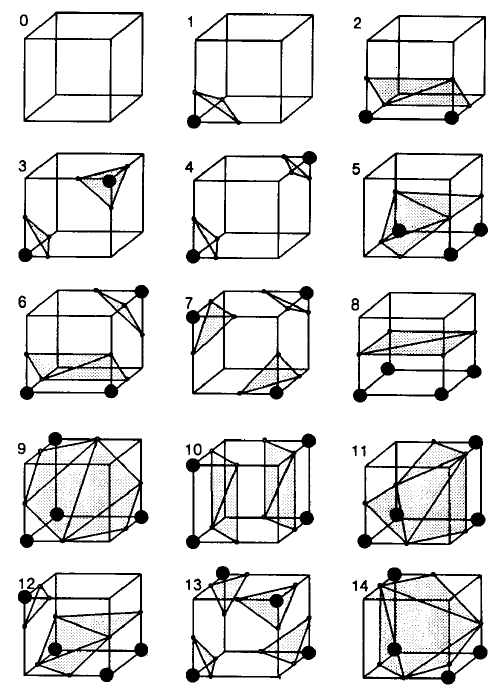
\includegraphics[scale=0.5]{przeciecia.PNG}
  \caption{Możliwe przecięcia sześcianu przez punkty \cite{lorensen1987marching}}   
  \label{fig:marchingCubesCut}
\end{figure}
Przecięcia punktów z sześcianami tworzą trójkąty, które później zostaną dodane do triangulacji. Należy zwrócić uwagę na to, że gęstość meshu na obiekcie poddanym triangulacji bezpośrednio zależy od długości boku sześcianu. Im jest on mniejszy, tym więcej będzie przecięć punktów z krawędziami, a co za tym idzie, więcej utworzonych trójkątów triangulacyjnych. Występują odmiany tej metody wprowadzające zmienną długość boku danego sześcianu \cite{shu1995adaptive}. Adaptacyjna metoda maszerujących sześcianów bada krzywiznę powierzchni wewnątrz sześcianów za pomocą wyznaczania wektorów normalnych utworzonych dla danych trójkątów. Jeśli wektory odchylone są w podobną stronę, oznacza to, że powierzchnia jest dostatecznie gładka. W przeciwnym wypadku sześcian dzielony jest na kolejne 8 sześcianów i algorytm jest powtarzany do momentu uzyskania odpowiedniej krzywizny powierzchni. Dzięki wykorzystaniu tej metody tworzona jest dokładniejsza triangulacja powierzchni względem początkowego algorytmu. Ponadto dzięki wykorzystaniu adaptacyjnej metody algorytm jest szybszy niż ten który by miał ustalona długość boku. Porównanie algorytmu maszerujących sześcianów oraz jej adaptacyjnej odmiany dla różnych ilości punktów znajduje się w tabeli ~\ref{tab:amcvsmc}.

\begin{table}[H]
\begin{center}
\caption{\label{tab:amcvsmc}Porównanie algorytmu MS oraz adaptacyjnych MS dla 7.4\cdot $10^6$ oraz 2.8\cdot $10^6$ punktów \cite{shu1995adaptive}.}
\begin{tabular}{ |c| c|c|c|c| }
 \hline
 {\small Metoda} & {\small MS}&{ \small AMS} & {\small MS}&{ \small AMS}\\ 
  \hline
     {\small Liczba punktów } & {\small  7.4\cdot $10^6$ } & {\small  7.4\cdot $10^6$ } & {\small  2.8\cdot $10^6$ } & {\small  2.8\cdot $10^6$ }   \\  
  \hline
     {\small Czas trwania } & {\small 331 s} & {\small 230 s}& {\small 164 s} & {\small 81 s}    \\  
  \hline
   {\small  Ilość trójkątów } & {\small 718964 } & {\small 299292 }& {\small 393606 } & {\small 102868 }  \\  
  \hline
\end{tabular}
\end{center}
\end{table}



\subsection{Ball pivoting algorithm}

Algorytm toczącej się kuli jest metodą służącą do rekonstrukcji powierzchni na podstawie chmury punktów. Został on zaproponowany przez Fausto Bernardini i pozostałych w 1999 roku \cite{bernardini1999ball}. BPA został stworzony by szybko i dokładnie odwzorowywać kształt powierzchni. Schemat postępowania programu, opiera się o kulę, która toczy się po powierzchni punktów. Z początku, wybierany jest pierwszy trójkąt triangulacyjny. Trzy punkty utworzą pierwszy trójkąt triangulacyjny, jeśli kula styka się tylko i wyłącznie z nimi. Gdy tocząc się ,kula natrafi na dodatkowy punkt, to zostaje on połączony z bokiem wcześniejszego trójkąta. Cały proces powtarza się do momentu, gdy kula pokona całą powierzchnię. Pomimo przejścia kuli przez całą powierzchnię, nie oznacza to, że ze wszystkich punktów zostanie utworzony mesh. Warto nadmienić, że głównym parametrem wpływającym na czas trwania algorytmu jest promień kuli. W większości przypadków, ustala się go na podstawie średniej odległości punktów od siebie. Jeśli promień będzie niedostatecznie duży, to kula może "wypaść" przez punkty, więc nie zostaną one połączone. Powstają wtedy dziury, które negatywnie wpływają na ostateczny wygląd meshu. Można je później załatać wykorzystując algorytmy interpolacji liniowej lub ponownie uruchomić algorytm BPA, tym razem z większym promienień i powtórzyć cały proces jeszcze raz. W efekcie czego większość dziur zostanie załatana. Wpłynie to jednak negatywnie na czas trwania algorytmu. Wizualizacja zasady działania algorytmu została przedstawiona na rysunku ~\ref{fig:bpaZasada}

\begin{figure}[H]
  \centering
  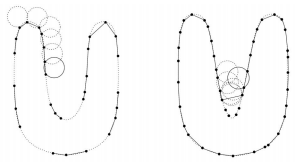
\includegraphics[scale=0.8]{bpa_zasada.PNG}
  \caption{Zasada działania algorytmu BPA \cite{bernardini1999ball}}   
  \label{fig:bpaZasada}
\end{figure}
Główną zaletą przy wykorzystaniu tego algorytmu jest fakt, że jego złożoność obliczeniowa zależy liniowo od ilości punktów w zbiorze. Jeśli dodamy dodatkowy punkt, to kula musi się przez niego przetoczyć kilka razy. Jednak cała struktura pozostałych punktów pozostaje niezmienna. Ten aspekt algorytmu stanowi największą odmianę względem triangulacją Delaunay'a. W triangulacji Delaunay'a, po dodaniu dodatkowego punktu cała struktura triangulacji może się zmienić. Ważną zaletą algorytmu jest możliwość regulacji promienia kuli R, im promień jest mniejszy, tym algorytm zajmie więcej czasu, ponieważ zetknie się z większą ilością punktów podczas toczenia. Zatem eksperymentując z długością promienia, można otrzymać zadowalająco dobre rezultaty w krótszym czasie. 



\endgroup




\renewcommand{\listtablename}{Spis tabel}
\renewcommand{\listfigurename}{Spis rysunków}
\addcontentsline{toc}{chapter}{Spis tabel}
\addcontentsline{toc}{chapter}{Spis rysunków}
\listoffigures
\listoftables


\addcontentsline{toc}{chapter}{Bibliografia}
\bibliography{references}
\bibliographystyle{ieeetr}
\end{document}
